\documentclass{ximera}

%\usepackage{todonotes}

\newcommand{\todo}{}

\usepackage{esint} % for \oiint
\ifxake%%https://math.meta.stackexchange.com/questions/9973/how-do-you-render-a-closed-surface-double-integral
\renewcommand{\oiint}{{\large\bigcirc}\kern-1.56em\iint}
\fi


\graphicspath{
  {./}
  {ximeraTutorial/}
  {basicPhilosophy/}
  {functionsOfSeveralVariables/}
  {normalVectors/}
  {lagrangeMultipliers/}
  {vectorFields/}
  {greensTheorem/}
  {shapeOfThingsToCome/}
  {dotProducts/}
  {partialDerivativesAndTheGradientVector/}
  {../productAndQuotientRules/exercises/}
  {../normalVectors/exercisesParametricPlots/}
  {../continuityOfFunctionsOfSeveralVariables/exercises/}
  {../partialDerivativesAndTheGradientVector/exercises/}
  {../directionalDerivativeAndChainRule/exercises/}
  {../commonCoordinates/exercisesCylindricalCoordinates/}
  {../commonCoordinates/exercisesSphericalCoordinates/}
  {../greensTheorem/exercisesCurlAndLineIntegrals/}
  {../greensTheorem/exercisesDivergenceAndLineIntegrals/}
  {../shapeOfThingsToCome/exercisesDivergenceTheorem/}
  {../greensTheorem/}
  {../shapeOfThingsToCome/}
  {../separableDifferentialEquations/exercises/}
  {vectorFields/}
}

\newcommand{\mooculus}{\textsf{\textbf{MOOC}\textnormal{\textsf{ULUS}}}}

\usepackage{tkz-euclide}
\usepackage{tikz}
\usepackage{tikz-cd}
\usetikzlibrary{arrows}
\tikzset{>=stealth,commutative diagrams/.cd,
  arrow style=tikz,diagrams={>=stealth}} %% cool arrow head
\tikzset{shorten <>/.style={ shorten >=#1, shorten <=#1 } } %% allows shorter vectors

\usetikzlibrary{backgrounds} %% for boxes around graphs
\usetikzlibrary{shapes,positioning}  %% Clouds and stars
\usetikzlibrary{matrix} %% for matrix
\usepgfplotslibrary{polar} %% for polar plots
\usepgfplotslibrary{fillbetween} %% to shade area between curves in TikZ
%\usetkzobj{all}
\usepackage[makeroom]{cancel} %% for strike outs
%\usepackage{mathtools} %% for pretty underbrace % Breaks Ximera
%\usepackage{multicol}
\usepackage{pgffor} %% required for integral for loops



%% http://tex.stackexchange.com/questions/66490/drawing-a-tikz-arc-specifying-the-center
%% Draws beach ball
\tikzset{pics/carc/.style args={#1:#2:#3}{code={\draw[pic actions] (#1:#3) arc(#1:#2:#3);}}}



\usepackage{array}
\setlength{\extrarowheight}{+.1cm}
\newdimen\digitwidth
\settowidth\digitwidth{9}
\def\divrule#1#2{
\noalign{\moveright#1\digitwidth
\vbox{\hrule width#2\digitwidth}}}




% \newcommand{\RR}{\mathbb R}
% \newcommand{\R}{\mathbb R}
% \newcommand{\N}{\mathbb N}
% \newcommand{\Z}{\mathbb Z}

\newcommand{\sagemath}{\textsf{SageMath}}


%\renewcommand{\d}{\,d\!}
%\renewcommand{\d}{\mathop{}\!d}
%\newcommand{\dd}[2][]{\frac{\d #1}{\d #2}}
%\newcommand{\pp}[2][]{\frac{\partial #1}{\partial #2}}
% \renewcommand{\l}{\ell}
%\newcommand{\ddx}{\frac{d}{\d x}}

% \newcommand{\zeroOverZero}{\ensuremath{\boldsymbol{\tfrac{0}{0}}}}
%\newcommand{\inftyOverInfty}{\ensuremath{\boldsymbol{\tfrac{\infty}{\infty}}}}
%\newcommand{\zeroOverInfty}{\ensuremath{\boldsymbol{\tfrac{0}{\infty}}}}
%\newcommand{\zeroTimesInfty}{\ensuremath{\small\boldsymbol{0\cdot \infty}}}
%\newcommand{\inftyMinusInfty}{\ensuremath{\small\boldsymbol{\infty - \infty}}}
%\newcommand{\oneToInfty}{\ensuremath{\boldsymbol{1^\infty}}}
%\newcommand{\zeroToZero}{\ensuremath{\boldsymbol{0^0}}}
%\newcommand{\inftyToZero}{\ensuremath{\boldsymbol{\infty^0}}}



% \newcommand{\numOverZero}{\ensuremath{\boldsymbol{\tfrac{\#}{0}}}}
% \newcommand{\dfn}{\textbf}
% \newcommand{\unit}{\,\mathrm}
% \newcommand{\unit}{\mathop{}\!\mathrm}
% \newcommand{\eval}[1]{\bigg[ #1 \bigg]}
% \newcommand{\seq}[1]{\left( #1 \right)}
% \renewcommand{\epsilon}{\varepsilon}
% \renewcommand{\phi}{\varphi}


% \renewcommand{\iff}{\Leftrightarrow}

% \DeclareMathOperator{\arccot}{arccot}
% \DeclareMathOperator{\arcsec}{arcsec}
% \DeclareMathOperator{\arccsc}{arccsc}
% \DeclareMathOperator{\si}{Si}
% \DeclareMathOperator{\scal}{scal}
% \DeclareMathOperator{\sign}{sign}


%% \newcommand{\tightoverset}[2]{% for arrow vec
%%   \mathop{#2}\limits^{\vbox to -.5ex{\kern-0.75ex\hbox{$#1$}\vss}}}
% \newcommand{\arrowvec}[1]{{\overset{\rightharpoonup}{#1}}}
% \renewcommand{\vec}[1]{\arrowvec{\mathbf{#1}}}
% \renewcommand{\vec}[1]{{\overset{\boldsymbol{\rightharpoonup}}{\mathbf{#1}}}}

% \newcommand{\point}[1]{\left(#1\right)} %this allows \vector{ to be changed to \vector{ with a quick find and replace
% \newcommand{\pt}[1]{\mathbf{#1}} %this allows \vec{ to be changed to \vec{ with a quick find and replace
% \newcommand{\Lim}[2]{\lim_{\point{#1} \to \point{#2}}} %Bart, I changed this to point since I want to use it.  It runs through both of the exercise and exerciseE files in limits section, which is why it was in each document to start with.

% \DeclareMathOperator{\proj}{\mathbf{proj}}
% \newcommand{\veci}{{\boldsymbol{\hat{\imath}}}}
% \newcommand{\vecj}{{\boldsymbol{\hat{\jmath}}}}
% \newcommand{\veck}{{\boldsymbol{\hat{k}}}}
% \newcommand{\vecl}{\vec{\boldsymbol{\l}}}
% \newcommand{\uvec}[1]{\mathbf{\hat{#1}}}
% \newcommand{\utan}{\mathbf{\hat{t}}}
% \newcommand{\unormal}{\mathbf{\hat{n}}}
% \newcommand{\ubinormal}{\mathbf{\hat{b}}}

% \newcommand{\dotp}{\bullet}
% \newcommand{\cross}{\boldsymbol\times}
% \newcommand{\grad}{\boldsymbol\nabla}
% \newcommand{\divergence}{\grad\dotp}
% \newcommand{\curl}{\grad\cross}
%\DeclareMathOperator{\divergence}{divergence}
%\DeclareMathOperator{\curl}[1]{\grad\cross #1}
% \newcommand{\lto}{\mathop{\longrightarrow\,}\limits}

% \renewcommand{\bar}{\overline}

\colorlet{textColor}{black}
\colorlet{background}{white}
\colorlet{penColor}{blue!50!black} % Color of a curve in a plot
\colorlet{penColor2}{red!50!black}% Color of a curve in a plot
\colorlet{penColor3}{red!50!blue} % Color of a curve in a plot
\colorlet{penColor4}{green!50!black} % Color of a curve in a plot
\colorlet{penColor5}{orange!80!black} % Color of a curve in a plot
\colorlet{penColor6}{yellow!70!black} % Color of a curve in a plot
\colorlet{fill1}{penColor!20} % Color of fill in a plot
\colorlet{fill2}{penColor2!20} % Color of fill in a plot
\colorlet{fillp}{fill1} % Color of positive area
\colorlet{filln}{penColor2!20} % Color of negative area
\colorlet{fill3}{penColor3!20} % Fill
\colorlet{fill4}{penColor4!20} % Fill
\colorlet{fill5}{penColor5!20} % Fill
\colorlet{gridColor}{gray!50} % Color of grid in a plot

\newcommand{\surfaceColor}{violet}
\newcommand{\surfaceColorTwo}{redyellow}
\newcommand{\sliceColor}{greenyellow}




\pgfmathdeclarefunction{gauss}{2}{% gives gaussian
  \pgfmathparse{1/(#2*sqrt(2*pi))*exp(-((x-#1)^2)/(2*#2^2))}%
}


%%%%%%%%%%%%%
%% Vectors
%%%%%%%%%%%%%

%% Simple horiz vectors
\renewcommand{\vector}[1]{\left\langle #1\right\rangle}


%% %% Complex Horiz Vectors with angle brackets
%% \makeatletter
%% \renewcommand{\vector}[2][ , ]{\left\langle%
%%   \def\nextitem{\def\nextitem{#1}}%
%%   \@for \el:=#2\do{\nextitem\el}\right\rangle%
%% }
%% \makeatother

%% %% Vertical Vectors
%% \def\vector#1{\begin{bmatrix}\vecListA#1,,\end{bmatrix}}
%% \def\vecListA#1,{\if,#1,\else #1\cr \expandafter \vecListA \fi}

%%%%%%%%%%%%%
%% End of vectors
%%%%%%%%%%%%%

%\newcommand{\fullwidth}{}
%\newcommand{\normalwidth}{}



%% makes a snazzy t-chart for evaluating functions
%\newenvironment{tchart}{\rowcolors{2}{}{background!90!textColor}\array}{\endarray}

%%This is to help with formatting on future title pages.
\newenvironment{sectionOutcomes}{}{}



%% Flowchart stuff
%\tikzstyle{startstop} = [rectangle, rounded corners, minimum width=3cm, minimum height=1cm,text centered, draw=black]
%\tikzstyle{question} = [rectangle, minimum width=3cm, minimum height=1cm, text centered, draw=black]
%\tikzstyle{decision} = [trapezium, trapezium left angle=70, trapezium right angle=110, minimum width=3cm, minimum height=1cm, text centered, draw=black]
%\tikzstyle{question} = [rectangle, rounded corners, minimum width=3cm, minimum height=1cm,text centered, draw=black]
%\tikzstyle{process} = [rectangle, minimum width=3cm, minimum height=1cm, text centered, draw=black]
%\tikzstyle{decision} = [trapezium, trapezium left angle=70, trapezium right angle=110, minimum width=3cm, minimum height=1cm, text centered, draw=black]


\title{Proportional Change}

\begin{document}

\begin{abstract}
linear
\end{abstract}
\maketitle



Two related measurements change proportionally when a change in one measurement is a constant multiple of the change in another measurement. \\

\begin{warning}

The values of the measurements are not contant multiples of each other. \\


The \textbf{\textcolor{red!70!black}{changes}} in the measurments are constant multiples of each other.

\end{warning}


The growth of the two measurements has a constant rate, a conversion factor. \\



There are many relationships between measurements that exhibit proportional changes.  







\subsection*{Proportional Changes}




\begin{example} Speed


Suppose a car is traveling on the highway at a constant speed of $60 \, mph$.


$\blacktriangleright$ Whenever the distance measurement \textbf{\textcolor{purple!85!blue}{changes}} by $60 \, miles$, the time measurement \textbf{\textcolor{purple!85!blue}{changes}} by $1 \, hour$. \\
$\blacktriangleright$ Whenever the time measurement \textbf{\textcolor{purple!85!blue}{changes}} by $1 \, hour$, the distance measurement \textbf{\textcolor{purple!85!blue}{changes}} by $60 \, miles$. \\




\begin{itemize}
\item When the time changes by $2$ hours, the distance changes by $\answer{120}$ miles. \\
\item When the time changes by $5$ hours, the distance changes by $\answer{300}$ miles. \\
\item When the time changes by $0.5$ hours, the distance changes by $\answer{30}$ miles. \\
\end{itemize}



We have a constant conversion factor of $\frac{60 \, miles}{1 \, hour}$ for converting time changes into distance changes. \\






\begin{itemize}
\item When the distance changes by $2$ miles, the time changes by $\answer{\frac{1}{30}}$ hours. \\
\item When the distance changes by $5$ miles, the time changes by $\answer{\frac{1}{12}}$ hours. \\
\item When the distance changes by $0.5$ miles, the time changes by $\answer{\frac{1}{120}}$ hours. \\
\end{itemize}



We have a constant conversion factor of $\frac{1 \, hour}{60 \, mile}$ for converting distance changes into time changes. \\




$\blacktriangleright$ One viewpoint is that, in this situation, $60 \, miles = 1 hour$.  When one change occurs, the other must occur as well.





\end{example} 









\begin{notation}  \textbf{\textcolor{red!70!black}{$\Delta$}} \\


Mathematics has a shorthand symbol for ``change''.  It is an uppercase Greek delta: $\Delta$

\end{notation}

\textbf{\textcolor{purple!85!blue}{$\blacktriangleright$}}  In the previous example, it might be more appropriate to say \textbf{\textcolor{purple!85!blue}{$\Delta 60 \, miles = \Delta 1 hour$}} . It is the change in the measurements that is proportional.




\begin{example} Temperature


Temperature can be measured in degrees Fahrenheit or degrees Celsius and these measurements change proportionally. 


$\blacktriangleright$ Whenever the Fahrenheit measurement changes by $9^{\circ}$, the Celsius measurement changes by $5^{\circ}$. \\
$\blacktriangleright$ Whenever the Celsius measurement changes by $5^{\circ}$, the Fahrenheit measurement changes by $9^{\circ}$. \\



Water freezes at $0^{\circ}$ C and $32^{\circ}$ F.  From here, if the Celsius measurement changes by $100^{\circ}$, then the Fahrenheit measurement changes by $180^{\circ}$.  $18$ each of $5$'s and $9$'s. We get water boiling at $100^{\circ}$ celsius and $212^{\circ}$ degrees.


In this situation, $\frac{\Delta 5^{\circ}C}{\Delta 9^{\circ}F}$ or just $\frac{5^{\circ}C}{9^{\circ}F}$ is the conversion factor from Fahrenheit change to Celsius change, and $\frac{9^{\circ}F}{5^{\circ}C}$ is the conversion factor from Celsius to Fahrenheit.






\end{example} 
















\subsection*{Rates}


Those conversions are examples of \textbf{rates}. 








\begin{definition} \textbf{\textcolor{green!50!black}{Rate}} \\

A \textbf{rate} is a ratio between two quantities with different units.   \\



We usually represent rates with fractions, although we also use phrases involving ``per'' or equalities.

\end{definition}


For us, rates measure how one quantity changes compared to the change in another quantity.











\begin{example} Speed


Suppose a car is traveling on the highway at a constant speed of $60 \, mph$.


$\blacktriangleright$ Whenever the distance measurement changes by $60 \, miles$, the time measurement changes by $1 \, hour$. \\
$\blacktriangleright$ Whenever the time measurement changes by $1 \, hour$, the distance measurement changes by $60 \, miles$. \\




If we compare these related measurement changes in a rate, then we get

\[
\frac{\Delta Distance}{\Delta Time} = \frac{60 \, miles}{1 \, hour} = 60 \,miles \, per \, hour
\]


\end{example} 



This example gives us the equation for linear motion: $Distance = Rate \times Time$, which we could represent here with a function.

\[
D(t) = R \cdot t =  \frac{60 \, miles}{1 \, hour} \cdot t
\]









\begin{example} Temperature


Temperature can be measured in degrees Fahrenheit or degrees Celsius and these measurements have a function relationship. This relationship has a special property.


$\blacktriangleright$ Whenever the Fahrenheit measurement changes by $9^{\circ}$, the Celsius measurement changes by $5^{\circ}$. \\
$\blacktriangleright$ Whenever the Celsius measurement changes by $5^{\circ}$, the Fahrenheit measurement changes by $9^{\circ}$. \\



Water freezes at $0^{\circ}$ C and $32^{\circ}$ F.  From here, if the Celsius measurement changes by $100^{\circ}$, then the Fahrenheit measurement changes by $180^{\circ}$.  $20$ each of $5$'s and $9$'s. We get water boiling at $100^{\circ}$ celsius and $212^{\circ}$ degrees.


If we compare these related measurement changes in a rate, then we get

\[
\frac{\Delta Degrees}{\Delta Celsius} = \frac{9^{\circ}F}{5^{\circ}C} \, \text{ or } \, \frac{\Delta Celsius}{\Delta Degrees} = \frac{5^{\circ}C}{9^{\circ}F}
\]


\end{example} 


This second example gives us the conversion between Fahrenheit change and Celsius change, which we could express with a function.  We just have to remember that $0^{\circ}C = 32^{\circ}F$.

\[
F(C) = 32 + \frac{9}{5} \cdot C
\]


The formula converts each change of $5$ in $C$ into a change of $9$ for $F$.







\begin{definition} \textbf{\textcolor{green!50!black}{Constant Rate of Change}} \\


A rate is a comparison of how measurements \textbf{\textcolor{purple!85!blue}{CHANGE}}. A rate is not a comparison of the measurement values, but a comparison of how they change. \\


Two measurements share a \textbf{constant rate of change} of $\tfrac{A}{B}$ if whenever measurement \#1 changes by $A$, then measurement \#2 changes by $B$ and vice versa, and this rate is not dependent on the amount of each measurement present.  The rate is the same throughout the situation.  It is a constant.




\end{definition}




\begin{idea}


The growth rate is a multiplier.


Example: Whenever measurement \#1 changes by $A$, then measurement \#2 changes by $B$.  Then $\frac{A}{B}$ is a multiplier.  

\[
B \cdot \frac{A}{B} = B
\]


The rate converts change in one measurement to the ``equal'' change in the other measurement.

\end{idea}





















\section*{Linear Functions}








\begin{definition} \textbf{\textcolor{green!50!black}{Linear Functions}} \\

Linear functions are those functions where the domain and range share a constant rate of change.  

\end{definition}


Each linear function has its own constant rate of change (growth rate). \\


Suppose $L$ is a linear function.  Let $a$ and $b$ be numbers in the domain of $L$.  Then $L(a)$ and $L(b)$ are the corresponding range values.

Since $L$ is a linear function, we know that $\frac{L(b) - L(a)}{b - a} = constant$.  And, this works for ANY two domain numbers.

Otherwise, it is not a linear function.







\begin{example} \textit{Constant Rate of Change}


Suppose $f$ is a function, which contains the pairs $(3, 7)$, $(5, 17)$, and $(6, 23)$.


The rate-of-change from $3$ to $5$ is $\answer{5}$.

The rate-of-change from $5$ to $6$ is $\answer{6}$.

\begin{question} 
$f$ is a linear function.
\begin{multipleChoice}
\choice {True}
\choice [correct]{False}
\end{multipleChoice}
\end{question}

\end{example}


Somewhere in history, $m$ became a popular choice for the constant rate of change of a linear function.



\[
\frac{L(b) - L(a)}{b - a} = m
\]





No matter which two numbers you select from the domain of $L$, the rate of change always turns out to be $m$.  Each linear function has its own $m$ - its own constant rate of change.






\begin{model} \textit{Mileage vs. Weight}

\textbf{How does the weight of a car affect its gas mileage?} \\



$392$ makes and models of automobiles manufactured between 1970 and 1982 were considered.  

\begin{itemize}
\item How many gallons of gasoline were used to travel $100$ miles?   (gallons)
\item What is the weight of the car?    ($1000$ pounds)
\end{itemize}


These pairings are plotted below.




\begin{center}
\desmos{4ysvvryemv}{400}{300}
\end{center}


We can see from the graph that this is not the graph of a function.  It is a data plot.\\


Our goal is to make predictions about other cars from this data.  Therefore, we would like a \textbf{\textcolor{purple!85!blue}{model}} for this data.  That is, we would like a function that approximates the data relationship.  The easiest model is a linear model.


A linear model would be a linear function whose graph does the best job a line can do of pretending to be the dots.  The line should pass through the ``middle of the dots''.

In the DESMOS window above, change the values of ``$m$'' and ``$b$'' to find such a line. \\

When you have your line, turn on the model found by DESMOS by clicking on the circle next to $y_1 \sim a_1 x + a_2$.


Source:   \textit{regressit.com}
\end{model}



\begin{question}


DESMOS found the linear model $y_1 = 0.450808 x_1 + 0.820606$ \\


The units of $x_1$ are $1000 \, lbs$. \\
The units of $y_1$ are $gallons$.



What are the units of $0.450808$?

\begin{multipleChoice}
\choice {$gallons$}
\choice {$pounds$}
\choice[correct] {$\frac{gallon}{pound}$}
\choice {$\frac{pound}{gallon}$}
\end{multipleChoice}


\end{question}








\begin{question}


DESMOS found the linear model $y_1 = 0.450808 x_1 + 0.820606$ \\


The units of $x_1$ are $1000 \, lbs$. \\
The units of $y_1$ are $gallons$.



Which is the correct statement?

\begin{multipleChoice}
\choice[correct] {For every $1000 \, pounds$ added to a car, an extra $0.450808 \, gallons$ of gas is needed to travel $100 \, miles$.}
\choice {Every added gallon of gas can carry $4508.08 \, pounds$ an additional $100 \, miles$.}
\end{multipleChoice}


\end{question}






































\subsection*{A Formula}  


Let $L$ be a linear function.  That means it has is own unique constant rate of change.  Let's call it $m$. \\

Let $(a, b)$ be one specific pair in $L$.\\


Let $(x, y)$ represent any other pair (all other pairs) in the function $L$. 

\begin{formula} \textbf{\textcolor{blue!55!black}{Slope}} 


Then the rate of change from $(a,b)$ to $(x, y)$ must equal $m$.


\[  \frac{y - \answer{b}}{x-\answer{a}} = m \]
\end{formula}


Clearing the denominator gives us the point-slope form for a line.






\begin{formula} \textbf{\textcolor{blue!55!black}{Point-Slope Form for a Line}} 


In practice, along with the slope, $m$, we almost always have a point on the line that is not an intercept $(a,b)$. Describing the other points on the line is much easier with the point-slope form of a line.


\[  (y - b) = m (x - a) \]
\end{formula}






Since $(a, b)$ is a pair in $L$, we know that $b = L(a)$.  And, since $(x, y)$ represents any other pair in $L$, we know that $y = L(x)$.  Replacing these in the equation for constant slope gives


\[  \frac{L(x) - L(a)}{x-a} = m \]


Clearing the denominator gives


\[  L(x) - L(a) = m (x-a) + L(a)     \]

Solving this for $L(x)$ gives

\[  L(x) = m (x-a) + L(a)     \]



\textbf{Note:} In advanced mathematics, a similar idea called \textit{linear maps} are required to include the pair $(0,0)$.  This would result in $L(0) = 0$. \\  
This is not required for Calculus. \\




\begin{example} \textit{A pair and a rate-of-change}


Suppose $W$ is a linear function with constant rate of change equal to $5$ and $(3, -1)$ is one pair in $W$.  \\

Create a formula for $W$.

\textbf{explanation}



The template $L(x) = m (x-a) + L(a)$ tell us that a formula for $W$ looks like 


\[  W(x) = 5 (x-3) + \left(\answer{-1}\right)     \]


\[  W(x) = 5 (x-3) - 1     \]

We could multiply this out and collect like terms and obtain the equivalent formula


\[  W(x) = \answer{5}x - \answer{16}   \]



Perhaps, we do not like $x$ as the variable for our formula.  Perhaps $v$ suits our situation better.

\[  W(v) = 5v - 16   \]


Or, $k$.

\[  W(k) = 5k - 16   \]


Or, $A$.

\[  W(A) = 5A - 16   \]


It is always advantageous to select a variable that is a nice reminder of the domain measurement.

\end{example}









\begin{example} \textit{Two Pairs}


Suppose $g$ is a linear function containing $(0, 6)$ and $(-2, -5)$.

Then the template: $L(x) = m (x-a) + L(a)$ will need a rate of change



\[  m = \frac{-5 - 6}{\answer{-2} - \answer{0}} = \frac{-11}{-2} = \frac{11}{2}  \]

A formula for $g$ is


\[  g(t) = \frac{11}{2} (t-0) + 6     \]


\[  g(t) = \frac{11}{2} t + 6    \]



\end{example}






























\subsection*{A Graph}




A linear function has a line as its graph.  The line includes a point for each pair in the function.  And, since it is a line, only two points are needed to draw the graph.  Any two distinct points will do.





\begin{example} \textit{A Line}


Let $g(k) = \frac{k}{2} - 4$ be a linear function with its natural domain. Draw a graph of $g$.


\textbf{explanation}


Let's select two random domain numbers: $-4$ and $6$.  The function values at these domain numbers are $g(-4) = \answer{-6}$ and $g(6) = \answer{-1}$.  Therefore, the points $(-4, -6)$ and $(6, -1)$ are on the graph, which is a line.  We'll plot the two points and draw the line through them.


Below is the graph of $y=g(k)$.


\begin{image}
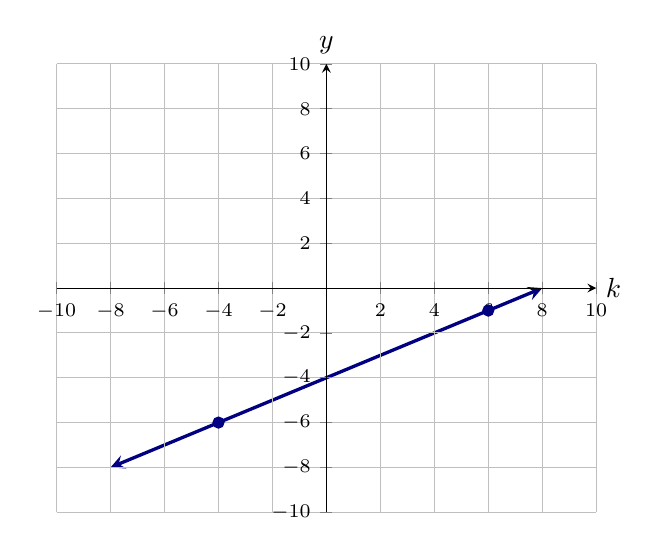
\begin{tikzpicture}
     \begin{axis}[
            	domain=-10:10, ymax=10, xmax=10, ymin=-10, xmin=-10,
            	axis lines =center, xlabel=$k$, ylabel=$y$, grid = major,
                ytick={-10,-8,-6,-4,-2,2,4,6,8,10},
                xtick={-10,-8,-6,-4,-2,2,4,6,8,10},
                ticklabel style={font=\scriptsize},
            	every axis y label/.style={at=(current axis.above origin),anchor=south},
            	every axis x label/.style={at=(current axis.right of origin),anchor=west},
            	axis on top,
          		]

        
        \addplot [draw=penColor, very thick, smooth, domain=(-8:8),<->] {0.5*x-4};

        \addplot[color=penColor,fill=penColor,only marks,mark=*] coordinates{(-4,-6)};
        \addplot[color=penColor,fill=penColor,only marks,mark=*] coordinates{(6,-1)};


    \end{axis}
\end{tikzpicture}
\end{image}




\end{example}










\begin{example} \textit{A Line}


Let $B(t)$ be a linear function.    Below is the graph of $y = B(t)$. From the graph obtain a formula for $B$.


\begin{image}
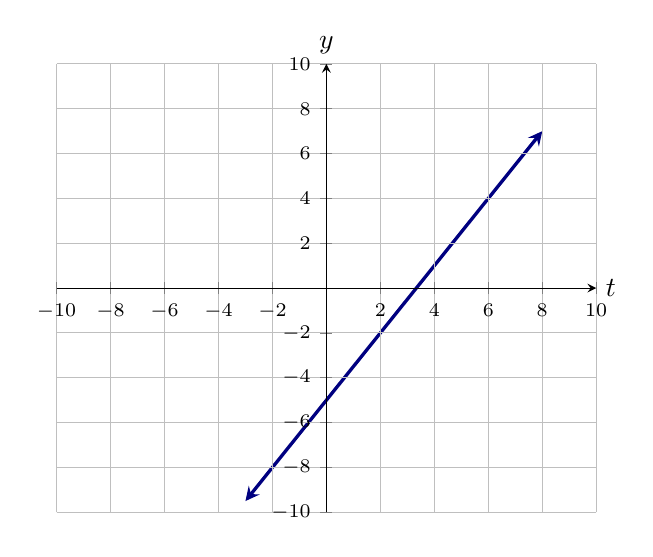
\begin{tikzpicture}
     \begin{axis}[
            	domain=-10:10, ymax=10, xmax=10, ymin=-10, xmin=-10,
            	axis lines =center, xlabel=$t$, ylabel=$y$, grid = major,
                ytick={-10,-8,-6,-4,-2,2,4,6,8,10},
                xtick={-10,-8,-6,-4,-2,2,4,6,8,10},
                ticklabel style={font=\scriptsize},
            	every axis y label/.style={at=(current axis.above origin),anchor=south},
            	every axis x label/.style={at=(current axis.right of origin),anchor=west},
            	axis on top,
          		]

        
        \addplot [draw=penColor, very thick, smooth, domain=(-3:8),<->] {(3/2)*x-5};

        %\addplot[color=penColor,fill=penColor,only marks,mark=*] coordinates{(-4,-6)};
        %\addplot[color=penColor,fill=penColor,only marks,mark=*] coordinates{(6,-1)};


    \end{axis}
\end{tikzpicture}
\end{image}


\textbf{explanation}


From the graph, we can approximate the points $(0, -5)$ and $(3.3, 0)$.  These give a slope of

\[  slope = \frac{0 - \left(\answer{-5}\right)}{\answer{3.3} - 0} = \frac{5}{3.3} (\approx 1.5)     \]


This would give the formula $B(t) = \frac{5}{3.3} (t - 0) - 5 = \frac{5}{3.3} t - 5$



\end{example}


We used the point $(0, -5)$ to create the equation.  We could also have used $(3.3,0)$.



$B(t) = \frac{5}{3.3} (t - 3.3) - 0 = \frac{5}{3.3} t - \frac{5}{3.3}\cdot 3.3 = \frac{5}{3.3} t -  5$ \\


Same equation.  You can use any point on the line.









\subsection*{Lines vs. Linear Functions}


When representing a linear function with a graph, we are expecting the horizontal axis to represent domain values and the vertical axis to represent function values. On the other hand, lines don't care about interpretation.\\


Depending on how we are using the graph will change how we interpret the information.  This idea will occur many times in mathematics. Context is everything.\\


\textbf{\textcolor{purple!85!blue}{Geometry:}} Graphs of lines don't care which axis is ``vertical'' and which axis is ``horizontal''.  The graph is just a collection of points whose coordinates satisfy the linear equation.  \\

\textbf{\textcolor{purple!85!blue}{Analysis:}} The situation changes once we wish to interpret one of the variables as a function of the other variable. Once we designate one of the variables as the dependent variable or the function, then its axis becomes the ``vertical'' axis.  The other axis measures the independent variable and represents the domain of the function. The domain is measured horizontally in the graph. \\


\textbf{Note:} This all works for all lines, except for vertical lines. All lines are graphs of linear functions, except vertical lines. \\



\begin{explanation}
When switching our thnking from geometry to functions, which variable is the function and which is the domain? \\

Either interpretation is ok.  The decision rests on the context.  \\

We can solve the equation for the function variable to obtain a formula.



Consider the linear equation $3 t + 2 y = 12$ \\

This equation can be rewritten as $y = \answer{\frac{-3}{2}} \, t + \answer{6}$.

This emphasizes that we are now thinking in terms of functions, we might write $y(t) = \tfrac{-3}{2} t + 6$.




We could just as easily have chosen $y$ as the domain variable and $t$ as the function variable.  In this case, $3 t + 2 y = 12$ can be rewritten as $t = \answer{\frac{-2}{3}} \, y + \answer{4}$.  We might write this as $t(y) = \tfrac{-2}{3} y + 4$




In either case, the function formula matches the ``$y = m \, x + b$'' template.  $\answer{m}$ is the slope of the line as well as the rate of change of the function.


\end{explanation}




\textbf{Note:}  ``$y = m \, x + b$'' is called the $y$-intercept form.  This is a nice compact form for a line equation or linear function.  However, it just disn't that useful.  We almost never get the intercept as information.  We almost always get a random point or pair.\\

It is much more helpful to use the point-slope form.





















\begin{onlineOnly}
\begin{center}
\textbf{\textcolor{green!50!black}{ooooo-=-=-=-ooOoo-=-=-=-ooooo}} \\

more examples can be found by following this link\\ \link[More Examples of Function Behavior]{https://ximera.osu.edu/csccmathematics/precalculus/precalculus/beginningOfBehavior/examples/exampleList}

\end{center}
\end{onlineOnly}





\end{document}
